\chapter{Phenomenological study of \runone four-top-quark production cross section limits}
\label{c:pheno}

The 95\% CL upper limit placed on the production of four top quarks at $\sqrt{s}=8$~TeV can be used to place constraints on new physics models which predict an enhancement in the \tttt production cross section. One particular model, which is described further in Chapter~\ref{c:theory}, is a simplified model of NMSSM in which a new particle, the sgluon, arises. The results of the search in the single lepton channel in Chapter~\ref{c:Run1} are used to place constraints on the mass and coupling of the sgluon alongside another complimentary search CMS search for new physics in the same-sign dilepton channel which also places a limit on SM four-quark-production using the same dataset at $\sqrt{s}=8$~TeV~\cite{Chatrchyan:2013fea}. The author personally made contributions to reinterpreting that latter search and hence it will be primarily discussed in this thesis. Full details of the combined analysis and particularly the reinterpretation of the single lepton analysis can be found in~\cite{Beck201548}.\\
The chapter is organised as follows: in Section~\ref{sec:simpModel} the simplified model which is considered for study is discussed while in Section~\ref{sec:reinterp} the methodology of reinterpreting the CMS same-sign dilepton search is discussed. The simulation of sgluon events is discussed in Section~\ref{sec:sgluonSim} and the analysis of the simulation in the reinterpretation is discussed in Section~\ref{sec:sgluonAna}. The results are given in Section~\ref{sec:sgluonResults} and conclusions in Section~\ref{sec:sgluonConc}.

\section{A simplified model for describing top-philic sgluons \label{sec:simpModel} }
In this section the simplified model of sgluon production and decay, which is a minimal extension of the SM, is described. The SM is supplemented by the Lagrangian in Eq.~\ref{eqn:sgluonLag} by adding a single real colour-octet field for the sgluon, $S^{a}$. The gauge interacions of a sgluon pair to gluons is represented by the QCD covariant derivative, $D_{\mu}S^a= \partial_{\mu} S^a + g_s f_{bc}{}^a G_\mu^b S^c$

\begin{equation}
 {\cal L}= \frac{1}{2}D_{\mu}S^aD^{\mu} S_a
          -\frac{1}{2}\ourmS^2 S^a S_a
          \label{eqn:sgluonLag}
\end{equation}



% \begin{equation}
%  D_{\mu}S^a= \partial_{\mu} S^a + g_s f_{bc}{}^a G_\mu^b S^c \ .
% \end{equation}
The strong coupling constant is represented by $g_s$, $f_{bc}{}^a$ are the structure
constants of the SU(3) gauge group and $G_\mu^a$ denotes the gluon field.
The effective Lagrangian in Eq.~\ref{eq:SingleSgluLag} represents the sgluon coupling to the SM degrees of freedom, where the first term represents the dimension-four coupling of the sgluon to a top-anti-top pair and the second term represents the sgluon's interaction with gluons.

\begin{equation}
 {\cal L}_{\rm eff}= \bar t\, T_a (\ourat^L P_L + \ourat^R P_R)\, t\, S^a
 +\frac{a_g}{\Lambda} d_a{}^{bc} S^a F_{\mu\nu, b} F^{\mu\nu, c}
 + {\rm h.c.} 
\label{eq:SingleSgluLag}\end{equation}

The dimensionless coupling of the sgluons to gluons is represented by ${a_g}$, which is a suppressed by the theory cutoff scale $\Lambda$. The coupling of the sgluon to the top quark is denoted by $\ourat^L$ and  $\ourat^R$ for the left-handed and right-handed couplings. In the fundamental representation, $d_a{}^{bc}$ is the symmetric structure constant and $P_{L}~(P_{R})$ is the left (right) parity projection operator. The generators of SU(3) are $T_a$.
Although sgluons can, in theory, couple via flavour-changing-neutral currents to different quark flavours, we only consider the interactions with top quarks which conserve flavour. This is motivated by R-symmetric supersymmetry with minimal flavour violation where only interactions of sgluons with top quarks and gluons are non-negligible.

In this model sgluons are top-philic, ie. they are only allowed to decay to \ttbar or to two gluons which is consistent with the class II scenarios in Ref.~\cite{Calvet:2012rk}. The benchmark values for the couplings and theory cut-off scale are:
% \begin{equation}
\begin{align}
 &\ourat^L = \ourat^R = \ourat = 1.5\times 10^{-3}\ , \quad
 a_g = 1.5\times 10^{-3},\nonumber \quad\text{and}\quad&\Lambda = 1~{\rm TeV}
 \label{eq:benchmark}
\end{align}
% \end{equation}

The $a_t$ coupling is varied in the range $[0.5,5]\times 10^{-3}$ and $a_g$ is varied in the range $[1.35, 1.65] \times 10^{-3}$. The mass of sgluons studied is in the range $[350,900]$~GeV. These values are consistent with ultraviolet-complete theories of supersymmetry which have coloured superpartners with mass in the range $[1,2]$~TeV.
\begin{figure}[h!]
\centering
    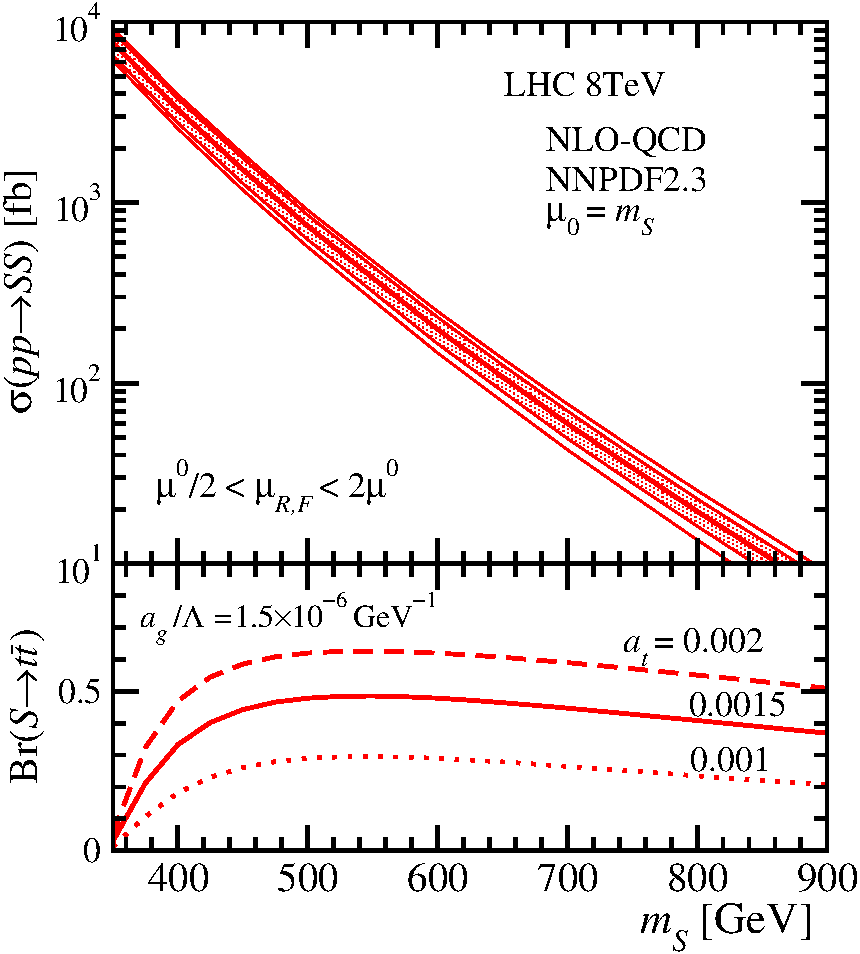
\includegraphics[width=0.7\textwidth]{images/Pheno/xsec.pdf}\\
    \caption{The top panel shows the $m_s$ dependence of the production of sgluon pairs from proton-proton collision at NLO with variations to the renormalisaton and factorisation scale by a factor of 1/2 and 2. The bottom panel shows the $m_s$ dependence of the branching fraction of the sgluon to a top-anti-top pair, Br$(S\rightarrow\ttbar)$, for different values of the coupling $a_t$ and a fixed value of $a_g$.}
    \label{fig:sgluonxsec}
\end{figure}

The simplified model discussed is consistent with an enhancement in the production of \tttt final states in proton-proton collisions, depending on the mass and couplings of the sgluon.

In Fig.~\ref{fig:sgluonxsec} the upper plot shows the dependence of the sgluon pair production cross section on the mass of the sgluon itself calculated at NLO accuracy in QCD~\cite{GoncalvesNetto:2012nt,Degrande:2014sta}. If sgluons were to have higher masses they would be less likely to be produced as it requires the quarks or gluons from the proton to have a high momentum fraction from the proton. The lower plot in Fig.~\ref{fig:sgluonxsec} shows the sgluon mass dependence of the branching fraction of a sgluon to a \ttbar pair for a range of $a_t$ coupling values. It can be seen that Br$(S\rightarrow\ttbar)$ increases from zero at twice the top quark mass.


\section{Reinterpretation of same-sign dilepton channel \label{sec:reinterp}}

The analysis by CMS of the same-sign dilepton channel at $\sqrt{s}=8$~TeV~\cite{Chatrchyan:2013fea} utilises the entire 2012 dataset of proton-proton collision of 19.6~\fbinv. The analysis is a collection of counting experiments that contain at least two same sign leptons and a number of jets. There are 28 signal regions which are categorised according to \njets, \nbtags, \HT, \MET and require the leptons to satisfy $\pt>20$~GeV and$|\eta|<2.4$.
Parameterisations are provided in this CMS paper which give the efficiency for reconstructing an object in simulation given generator-level information. These include:
% The efficiency curves for reconstructing an object in the detector given generator-level information are shown in Fig.~\ref for:
\begin{itemize}
\item The reconstruction of jets with respect to generator-level jet \pt ($\varepsilon_{jet}$)
\item The b-tagging of b-quark jets by the CSV algorithm with respect to generator-level jet \pt ($\varepsilon_{b}$)
\item The reconstruction of \HT with respect to generator-level \HT ($\varepsilon_{H_T}$)
\item The reconstruction of muons and electrons with respect to generator-level lepton \pt ($\varepsilon_{\mu}$, $\varepsilon_{e}$)
\item The reconstruction of \MET with respect to generator-level \MET ($\varepsilon_{\MET}$) 
\end{itemize}
as shown in Fig.~\ref{fig:effGraphs}.

\begin{figure}[ht!]
\begin{center}
% \subfloat{
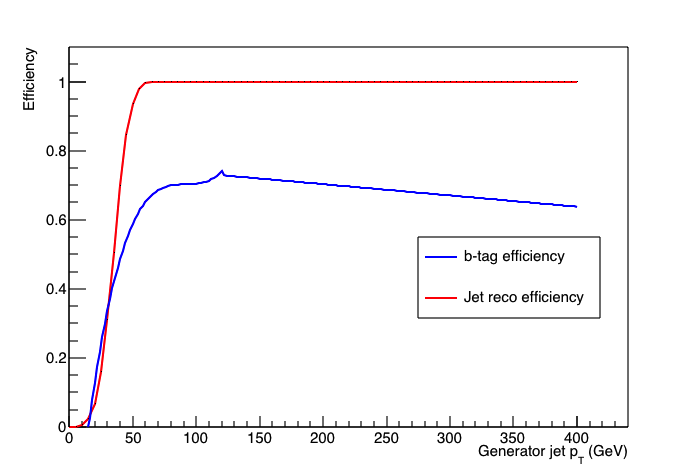
\includegraphics[width=0.49\textwidth]{images/Pheno/BTagEff.png}
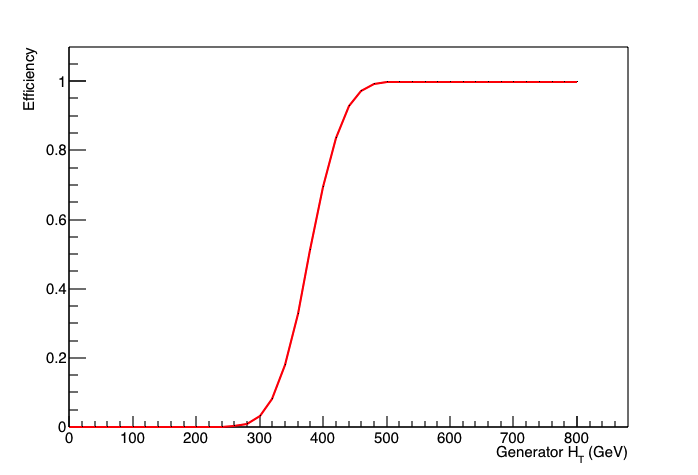
\includegraphics[width=0.49\textwidth]{images/Pheno/HTEff.png}\\
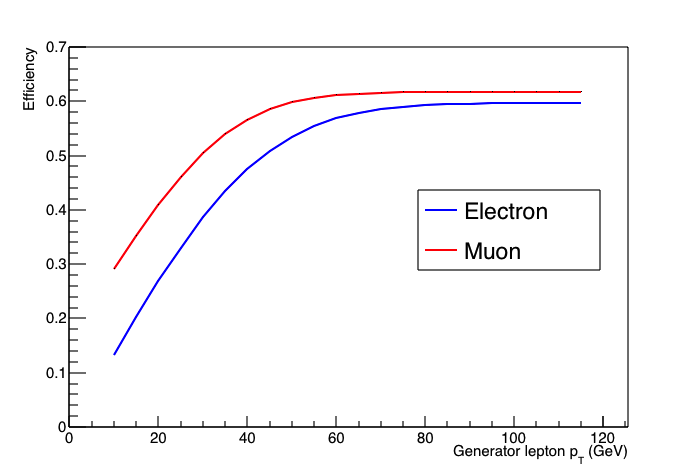
\includegraphics[width=0.49\textwidth]{images/Pheno/LeptonEff.png}
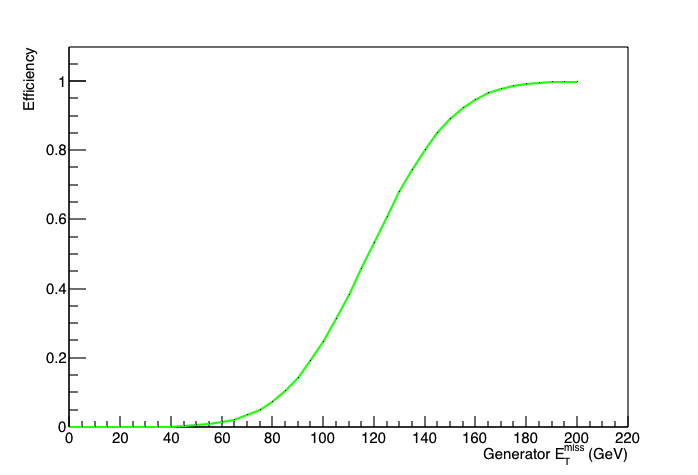
\includegraphics[width=0.49\textwidth]{images/Pheno/METEff.png}
% }
% \hspace{0.2cm}
\end{center}
\caption{Selection efficiencies for the reconstruction of jets and for b-tagging b-quark jets (top-left), for reconstructing \HT (top-right), for reconstructing muons and electrons (bottom-left) and for reconstructing \MET (bottom-right). Adapted from~\cite{Chatrchyan:2013fea}.}
\label{fig:effGraphs}
\end{figure}
Signal region 28 (SR28) was chosen to reinterpret as it closely corresponds to the \tttt signature and it can be fully emulated using the parameterisations of selection efficiency given in the paper. 
The requirements of SR28 are \njets$\geq4$, \nbtags$\geq2$, \HT$>400$~GeV, \MET$>$120~GeV and two same-sign leptons with \pt$>20$~GeV and $|\eta|<2.4$. Events which contain any additional leptons which form an opposite-sign-same-flavour (OSSF) pair with one of the signal leptons is vetoed if the invariant mass of the OSSF (M$_{\ell\ell}$) satisfies either M$_{\ell\ell}<12$~GeV or $76<$M$_{\ell\ell}<106$~GeV. This is to replicate the veto in the CMS search for events which may contain a low mass bound state or a Z boson.
It is not possible to combine the results from multiple signal regions without knowledge of the correlation of the uncertainties on the background. \\
The efficiency for obtaining at least 2 b-tagged jets, $\varepsilon_{\geq\text{2b-tags}}$, can be calculated using Eq.~\ref{eqn:2btags} where the probability, $P_{i}$, is for reconstructing a b-jet in this case. $P_{i}$ is the product of the probability to reconstruct a jet$_{i}$ and to tag it as b-jet, $\varepsilon_{jet} \times varepsilon_{b}$ which can be determined from the parameterisations of the curves in Fig.~\ref{fig:effGraphs} (top-left). A uniform efficiency for light quarks to be tagged as b-jet of $1\%$ is included to replicate the same-sign dilepton study.


\begin{equation}
w(\geq2~b~tags) = 1 - w(0) - w(1)
\label{eqn:2btags}
\end{equation}

\begin{equation}
w(0) = \prod_{i} ( 1 - P_{i})
\label{eqn:0btags}
\end{equation}


\begin{equation}
w(1) = \sum_{i}\left[P_{i}\prod_{j} ( 1 - P_{j})\right]~;~j\neq~i
\label{eqn:1btags}
\end{equation}

The efficiency for obtaining one same-sign dilepton pair in an event, $\varepsilon_{\geq1 \text{SS2L}}$ can be obtained by using Eq.~\ref{eqn:al1} where the weight for obtaining $\geq2$ same-sign positive or negative leptons, $ w(\geq2~l^{+})$ or  $ w(\geq2~l^{-})$, can be calculated using~\ref{eqn:2btags} along with the probabilities from the parameterisation of the muon and electron efficiency curves, ($\varepsilon_{\mu}$~\&~$\varepsilon_{e})$, in Fig.~\ref{fig:effGraphs} (bottom-left).

\begin{equation}
\varepsilon_{\geq1 \text{SS2L}} = 1 - \left[1-w(\geq2~l^{+})\right]\left[1-w(\geq2~l^{-})\right]
\label{eqn:al1}
\end{equation}

From the derived efficiencies for obtaining a specific \HT and \MET per event as well as $\geq2$~b tags and $\geq1$~SS dilepton pair, an overall event weight can be calculated using equation~\ref{eqn:phenoWeights}.

\begin{equation} \label{eqn:phenoWeights}
  w_{\rm event} = \varepsilon_{H_T} \times  \varepsilon_{\MET} \times
    \varepsilon_{\geq\text{2b-tags}} \times \varepsilon_{\geq1 \text{SS2L}} \ ,
\end{equation}

\section{Simulation of sgluon events \label{sec:sgluonSim}}
The \MGfive~\cite{Alwall2014} software package was used to simulate sgluon pair production with exclusive decays to top quarks at $\sqrt{s}=8$~TeV. \PYTHIAsix~\cite{pythia} was used to perform the hadronisation. The jet clustering was performed using the \antikt clustering algorithm in the \FASTJET package with a distance parameter of R$~=0.5$ and \pt$>5$ which is consistent with the same-sign analysis.

A sample of standard model four top quark events was also simulated using \MGfive and \PYTHIAsix. A signal efficiency for these events passing the SR28 selection was $0.6\%$ which can be compared to the $0.49\%$ signal acceptance listed in the same-sign analysis paper. These two numbers are agree within the $30\%$ uncertainty quoted for the analysis.

Sgluon events were simulated for a number of sgluon mass points, $m_{S}$, between $350 \geq m_{S} \geq 1000$~GeV and in the range of coupling to the top quark, $\alpha_{t}$, of $0.5 \times 10^{-3}\geq \alpha_{t} \geq 5 \times 10^{-3}$.

\section{Analysis \label{sec:sgluonAna}}

The \MADAN framework~\cite{Conte2013222} is used to perform the analysis. Using Eq.~\ref{eqn:phenoWeights} one can obtain the fraction of events which pass the selection and hence the signal efficiency for each sgluon ($m_{S},\alpha_{t}$) point. The number of sgluon events, $n^{S}_{events}$, which would be found in the same-sign analysis are obtained using Eq.~\ref{eqn:equivEvents}, where $\varepsilon\left(m_{S},\alpha_{t}\right)$ is the signal efficiency, $\sigma\left(m_{S},\alpha_{t}\right)$ is the cross section and $K_{NLO}\left(m_{S},\alpha_{t}\right)$ is a factor for the ratio of the NLO to LO cross section for that mass and coupling point. The luminosity, $\mathcal{L}$, is taken from the analysis to be 19.6~\fbinv. Rather than running the analysis in \MADAN for every coupling point, a nominal coupling can be provided and the program will produce weights, $F^{\alpha_{t}}\left(m_{S},\alpha_{t}\right)$ for each alternative coupling, where $F^{\alpha_{t}}\left(m_{S},\alpha_{t}\right) = 1$ for the nominal case.

\begin{equation}
n^{S}_{events}\left(m_{S},\alpha_{t}\right) = \varepsilon\left(m_{S},\alpha_{t}\right)\times \sigma\left(m_{S},\alpha_{t}\right) \times K_{NLO}\left(m_{S},\alpha_{t}\right) \times \mathcal{L}\times F^{\alpha_{t}}\left(m_{S},\alpha_{t}\right)
\label{eqn:equivEvents}
\end{equation}

This gives the number of sgluon events for each mass and coupling point in the chosen range, which then needs to be compared to the CMS analysis. CMS obtained 2 (2.21) event observed (expected) in SR28. This is converted to an $95\%$ C.L. upper limit of 4.68 (4.89) events observed (expected) by using the asymptotic \CLS method implemented in the \ROOSTAT package where the uncertainty of $30\%$ on the signal yield was assumed. Hence regions of the $\left(m_{S},\alpha_{t}\right)$ plane where $n^{S}_{events}$ is expected to be larger than 4.68 events can be excluded.


\section{Results \label{sec:sgluonResults}}

% Figure~\ref{fig:dilep2D} shows the number of events depending on the mass of the sgluon and it's coupling to the top quark. A contour is shown in red where the number of events is equal to 4.68 and hence any phase space point which has more events than this can be excluded.


% \begin{figure}[h!]
% \centering
%     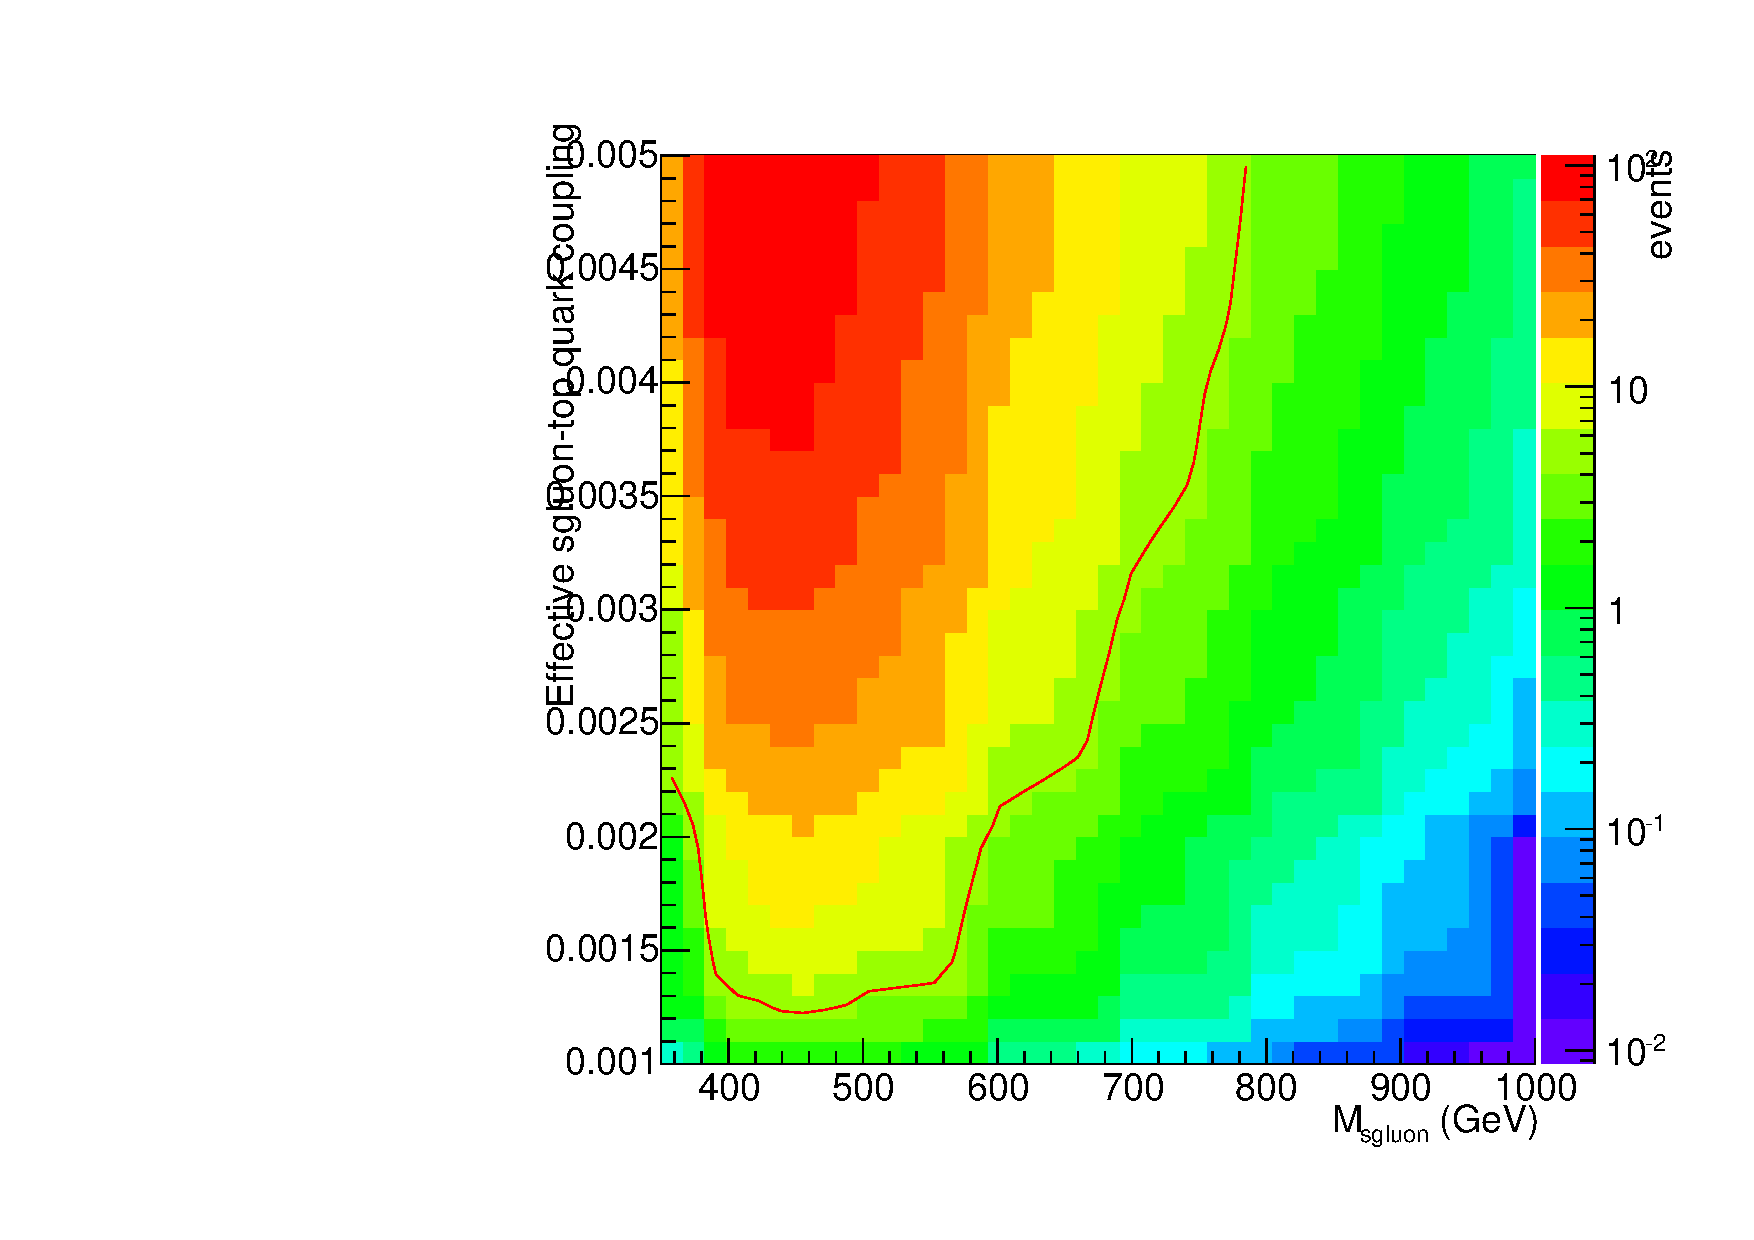
\includegraphics[width=0.7\textwidth]{images/Pheno/SG_nEvents2D.pdf}\\
%     \caption{Contours showing the number of expected events for a sgluon model with $m_{S}$, and coupling to the top quark, $\alpha_{t}$. The red lines show the $95\%$ C.L. upper limit on the number of events from the CMS SS dilepton analysis.}
%     \label{fig:dilep2D}
% \end{figure}

% This is developed further in Fig.~\ref{fig:sgluonExclusion} where the CMS single lepton analysis from~\cite{Chatrchyan:2013fea,Beck201548} is also included in the plot. The solid lines show the exclusion boundary for a fixed value of $a_{g}/\lambda = 1.5 \times 10^{-6}$~GeV$^{-1}$ and the dashed lines show a variation of $a_{g}$ by $\pm 10\%$. 
% In the mass region from 400 to 500~GeV sgluon models with couplings down to 0.0006 where the cross section of $\sigma( pp \rightarrow SS \rightarrow \tttt)$ is 
% maximal. The sensitivity worsens at low mass values due to the decreasing branching ratio, $\mathcal{B}\left(S\rightarrow~\ttbar \right)$, and at higher 
% mass values due to the decreasing cross section $\sigma( pp \rightarrow SS)$.
% The dilepton analysis is more constraining as it does not depend on event kinematics. It constrains up to $ m_{S} = 750$~GeV.


Figure~\ref{fig:sgluonExclusion} shows the exclusion boundary for the dilepton analysis where the number of events exceeds the CMS 95$\%$ C.L. limit in the exclusion zone. The CMS single lepton analysis from~\cite{Chatrchyan:2013fea,Beck201548}, is also included in the plot. The single lepton analysis uses a simplified Matrix Element Method to quantify how SM-like the sgluon event kinematics are for each mass and coupling point. The solid lines show the exclusion boundary for a fixed value of $a_{g}/\Lambda = 1.5 \times 10^{-6}$~GeV$^{-1}$ and the dashed lines show the change in the limit due to a variation of $a_{g}$ by $\pm 10\%$. 
In the mass region from 400 to 500~GeV sgluon models with couplings down to $6\times10^{-4}$ where the cross section of $\sigma( pp \rightarrow SS \rightarrow \tttt)$ is 
maximal. The sensitivity worsens at low mass values due to the decreasing branching ratio, $\mathcal{B}\left(S\rightarrow~\ttbar \right)$, and at higher mass values due to the decreasing cross section $\sigma( pp \rightarrow SS)$.
The dilepton analysis is more constraining as it does not depend on event kinematics. It constrains up to $ m_{S} = 750$~GeV at $a_t=5\times10^{-3}$ compared to around $ m_{S} = 750$~GeV for the single lepton channel. \fxnote{say more?}

\begin{figure}[h!]
\centering
    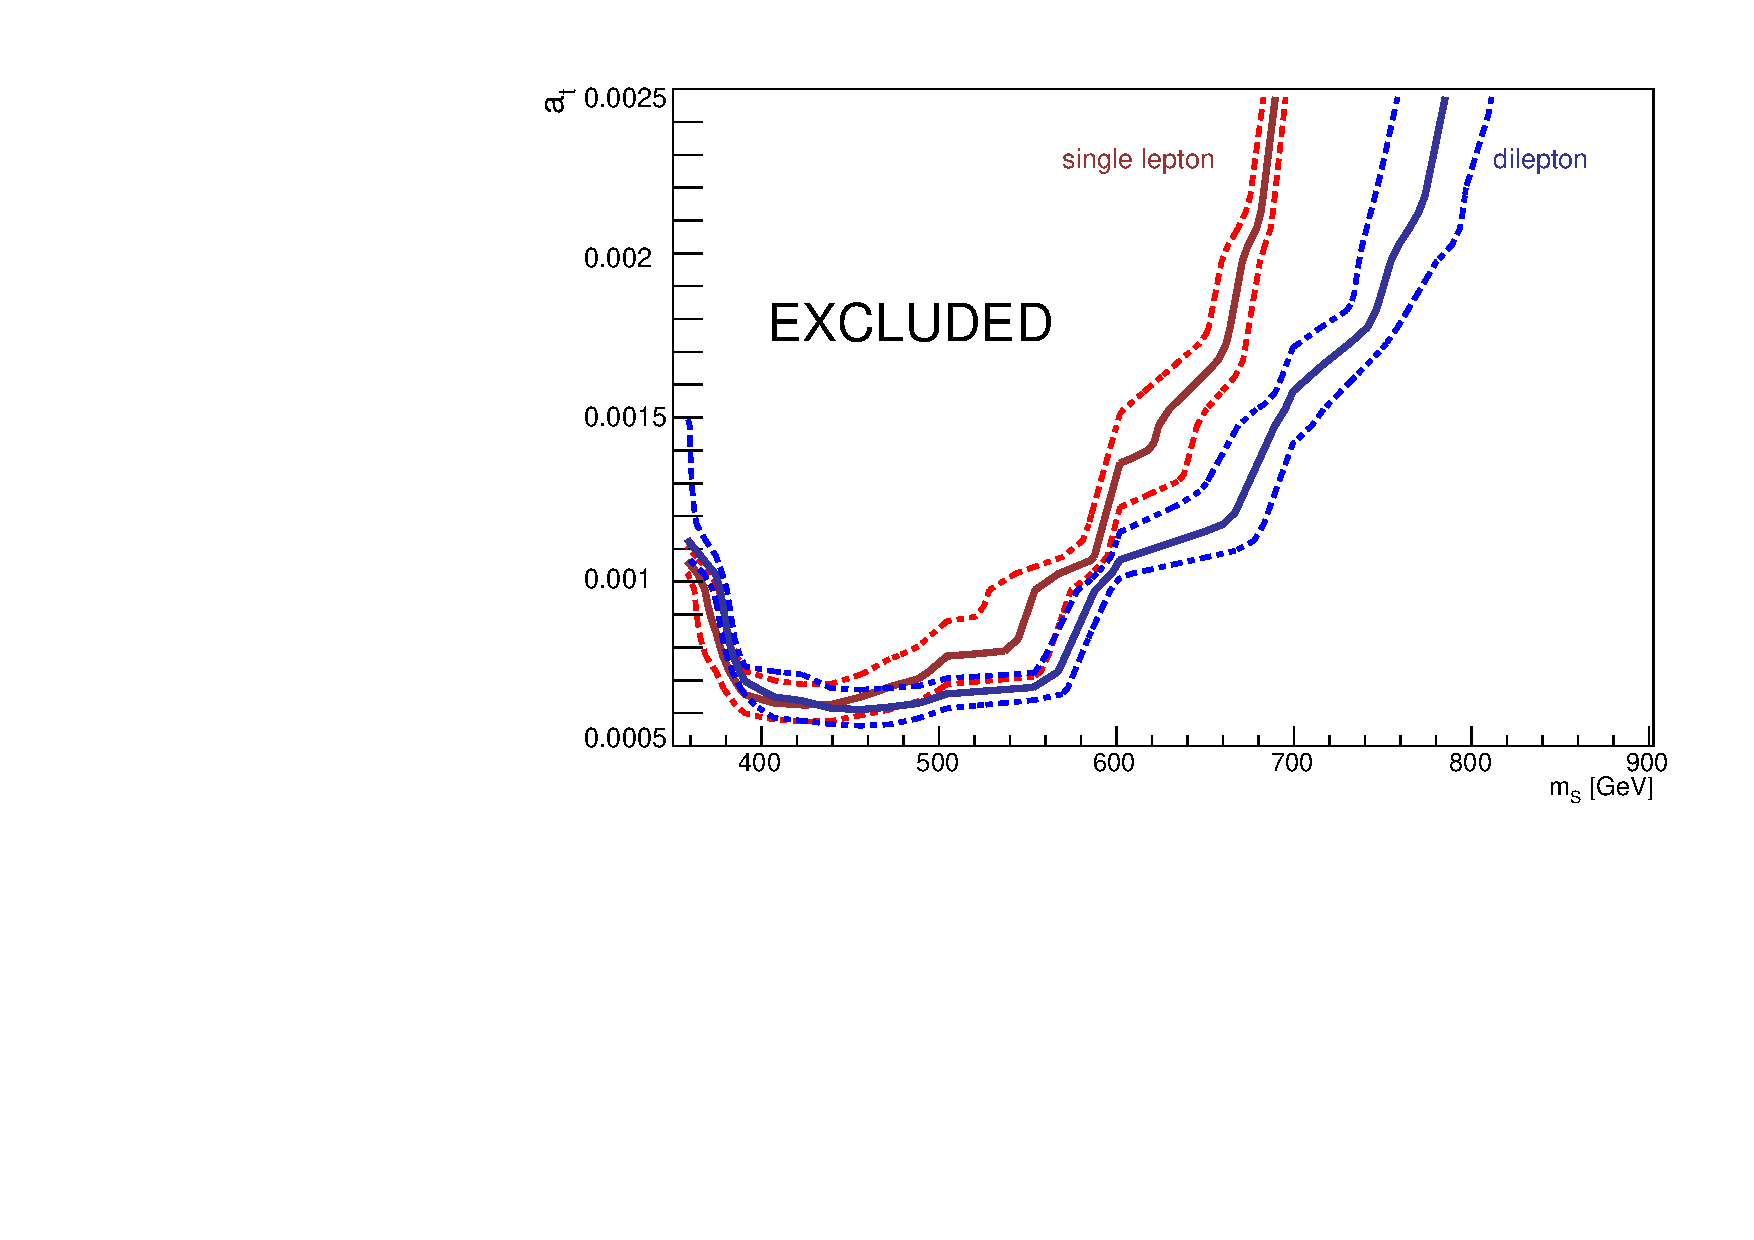
\includegraphics[width=0.9\textwidth]{images/Pheno/exclusion_agVariations.pdf}\\
    \caption{Solid lines show the exclusion boundary for a sgluon mass, $m_{S}$, and coupling to the top quark, $\alpha_{t}$, at $a_{g}/\Lambda = 1.5 \times 10^{-6}$~GeV$^{-1}$ and dashed lines show the results with a $\pm 10 \%$ variation in $a_{g}$}
    \label{fig:sgluonExclusion}
\end{figure}

\section{Conclusion \label{sec:sgluonConc}}

A simplified model approach has been used to described the dynamics of top-philic sgluons where the parameter space of $(m_{S}, a_{t}, a_{g}/\Lambda)$ has been explored. Two analyses, which set limits on the four-top-quark cross section, are used to place constraints on the phase space regions where sgluons may exist. The dilepton analysis is more powerful at excluding $m_{S}$ up to 700~GeV for the benchmark scenario of $a_{t}=1.5\times10^{-3}$, which is a typical value in the NMSSM for superpartners that have masses around 1-2~TeV. For $a_{t}<0.75\times10^{-3}$ the sgluon mass range of $400<m_{S}<580$~GeV is excluded. Varying $a_{g}$ by $10\%$ from it's benchmark value of $a_{g}/\Lambda = 1.5 \times 10^{-6}$~GeV$^{-1}$ does not have a significant impact on the result.